\documentclass[11pt]{report}
\usepackage[french]{babel}
\usepackage[utf8]{inputenc}
\usepackage[T1]{fontenc}
\usepackage[top = 2cm, bottom = 2cm, left = 1cm, right = 1cm]{geometry}
\usepackage{fancyvrb}
\usepackage{mathalfa}
\usepackage{amsfonts}
\usepackage[table]{xcolor}
\usepackage{amsmath}
\usepackage{graphicx}
\usepackage{listings}
\usepackage{color}
\usepackage{comment}
\usepackage{times}

\definecolor{brown2}{rgb}{0.5,0.2,0}

\lstset
{
	morestring=[b]",
	backgroundcolor=\color{cyan!10},
	basicstyle=\small\tt,
	breakatwhitespace=false,
	breaklines=true,      
	keepspaces=true,  
	keywords = [1]{foaf, rdf, @prefix},
	keywordstyle = [1]\color{blue},  
	keywords = [2]{type, knows},
	keywordstyle = [2]\color{brown2},
	keywords = [3]{td5},
	keywordstyle = [3]\color{red},   
	numbers=left,   
	numbersep=1em,          
	numberstyle=\tiny\color{black},       
	showspaces=false,                
	showstringspaces=false,          
	showtabs=false,           
	stepnumber=1,     
	stringstyle = \color{green},
	tabsize = 4
}

\begin{document}

\noindent
\textbf{Hachem BENYAHIA}
~\\
\textbf{Cristian GHITU}

~\\
\begin{center}
\section*{Compte-rendu IA04 - TD6 ~\\ Requêtes SPARQL}

~\\
\rule{\textwidth}{1pt}
\end{center}

~\\\\
\textbf{1. Rendre la base de connaissance créée durant les TDs 5 et 6.}

~\\
\begin{lstlisting}
@prefix				geo						<http://linkedgeodata.org/triplify/>.

td5:randomTopic1 	rdf:type 				foaf:topic.	
td5:randomTopic2	rdf:type 				foaf:topic.	
td5:randomTopic3	rdf:type 				foaf:topic.	

td5:a				rdf:type				foaf:Person;
					foaf:firstName			"A";
					foaf:family_name		"AA";

					foaf:knows				td5:b;
					foaf:knows				td5:c;
					foaf:knows				td5:d;

					foaf:topic_interest		td5:randomTopic1;
					foaf:topic_interest		td5:randomTopic2;
					foaf:topic_interest		td5:randomTopic3;
					
					foaf:topic_interest		geo:node1363947712.

td5:b				rdf:type				foaf:Person;
					foaf:firstName			"B";
					foaf:family_name		"BB";

					foaf:knows				td5:a;
					foaf:knows				td5:c;
					foaf:knows				td5:d;

					foaf:topic_interest		td5:randomTopic1;
					foaf:topic_interest		td5:randomTopic2;
					foaf:topic_interest		td5:randomTopic3;
					
					foaf:topic_interest		geo:node1363947712.
				
td5:c				rdf:type				foaf:Person;
					foaf:firstName			"C";
					foaf:family_name		"CC";

					foaf:knows				td5:a;
					foaf:knows				td5:b;
					foaf:knows				td5:e;

					foaf:topic_interest		td5:randomTopic1;
					foaf:topic_interest		td5:randomTopic2;
					foaf:topic_interest		td5:randomTopic3;
					
					foaf:topic_interest		geo:node1363947712.
					
td5:d				rdf:type				foaf:Person;
					foaf:firstName			"D";
					foaf:family_name		"DD";

					foaf:knows				td5:a;
					foaf:knows				td5:b;
					foaf:knows				td5:c;

					foaf:topic_interest		td5:randomTopic1;
					foaf:topic_interest		td5:randomTopic2;
					foaf:topic_interest		td5:randomTopic3;
					
					foaf:topic_interest		geo:node1363947712.
					
td5:e				rdf:type				foaf:Person;
					foaf:firstName			"E";
					foaf:family_name		"EE";

					foaf:knows				td5:b;
					foaf:knows				td5:c;
					foaf:knows				td5:d;

					foaf:topic_interest		td5:randomTopic1;
					foaf:topic_interest		td5:randomTopic2;
					foaf:topic_interest		td5:randomTopic3;
					
					foaf:topic_interest		geo:node1363947712.
\end{lstlisting}

\newpage
\noindent
\textbf{2. Donner l'architecture agent, les behaviours et un exemple de message échangés lors de la réponse envisagée à la question de l'étape 4.}

~\\
\begin{figure}[h]
\centering
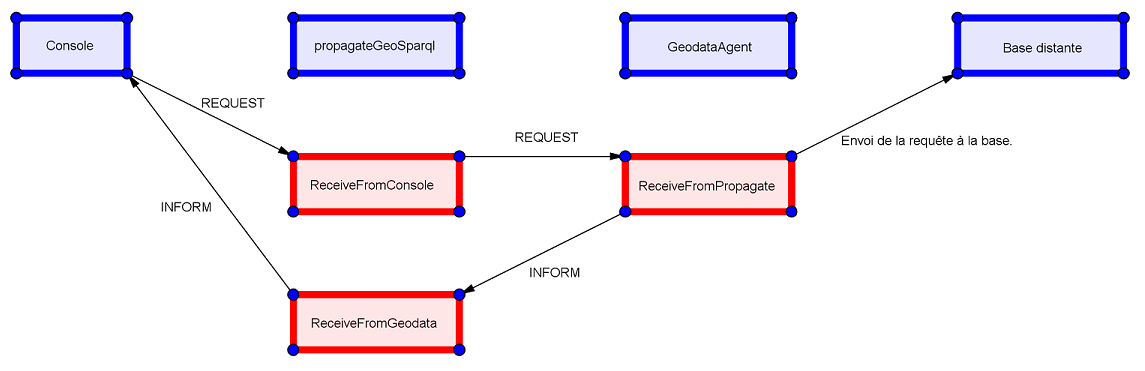
\includegraphics[width = \textwidth]{img/agents.png}
\caption{Architecture agent et behaviours.}
\end{figure}

~\\
\begin{figure}[h]
\centering
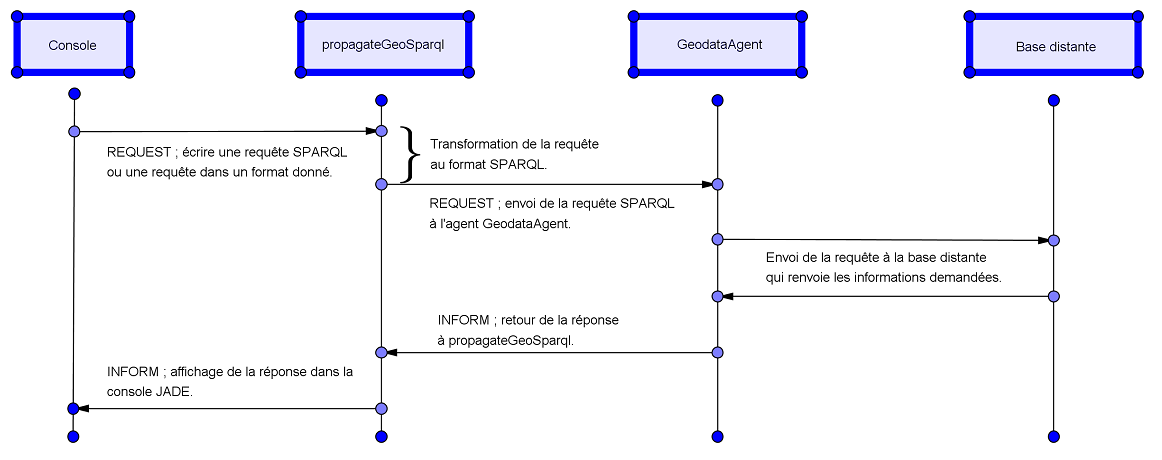
\includegraphics[width = \textwidth]{img/messages.png}
\caption{Exemple de messages échangés.}
\end{figure}

\end{document}